\documentclass[a4paper,11pt]{article}

\usepackage{jcappub}
\usepackage{txfonts}
\usepackage{threeparttable}
\usepackage{aas_macros}
\usepackage{graphicx}
\usepackage{subfigure}
\usepackage{url}


\title{Precision cosmology with time delay lenses: high resolution imaging requirements}
%\title{Cosmology with time delay lenses. High resolution imaging requirements}
\author[1]{Xiao-Lei Meng,}
\author[1,2]{Tommaso Treu,}
\author[1,2]{Adriano Agnello,}
\author[3]{Matthew W.~Auger,}
\author[1,2]{Kai Liao,}
\author[4]{Philip J. Marshall}

\affiliation[1]{Department of Physics, University of California, Santa Barbara, CA 93106, USA}
\affiliation[2]{Physics and Astronomy Building, 430 Portola Plaza, Box 951547, Los Angeles, CA 90095-1547, USA}
\affiliation[3]{Institute of Astronomy, UK}
\affiliation[4]{Kavli Institute for Particle Astrophysics and Cosmology, Stanford University, 452 Lomita Mall, Stanford, CA 94305, USA}

\emailAdd{xlmeng919@gmail.com}

\date{Accepted . Received }

\abstract{
Gravitational time delays are a powerful probe of cosmology, provided
that the gravitational potential of the main deflector can be modeled
with sufficient precision. Recent work has shown that this can be
achieved by detailed modeling of the host galaxies of lensed
quasars. The distortion of the images as measured over large number of
pixels provides tight constraints on the difference between the
gravitational potential between the two quasars, and thus on cosmology
in combination with the measured time delay. We carry out a systematic
exploration of the high resolution imaging required to eploit the
thousands of lensed quasars that will be discovered by current and
upcoming surveys with the next decade. Specifically we simulate
realistic lens systems as imaged by the Hubble Space Telescope (HST),
James Webb Space Telescope (JWST), ground based adaptive optics images
taken with Keck or the Thirty Meter Telescope (TMT). We compare the
performance of these pointed observations with that of images taken by
the Euclid-VIS, Wide-Field Infrared Survey Telescope (WFIRST) and
Large Synoptic Survey Telescope (LSST) surveys. Using as our metric
the precision with which the slope of the mass density profile for the
main deflector can be measured \textbf{we find that...}  }

\keywords{}

\begin{document}
\maketitle
\flushbottom


\section{Introduction}
\textbf{[TT to put introfirst here; introduce `informative pixels' that will be referred to in Sect.s 2 and 3; mention that we're basically observing how radial magnification changes across the lens, so that we need to understand how that is affected by PSF, pixel-size, and S/N ratio.]}

In the past few years, gravitational time delays have emerged as a...

This paper is organized as follows. We first introduce a variety of instrument informations in Section 2. Next, we briefly summarize the lens sample used in this work in Section 3 and show how to reconstruct lens models
as imaged by these instruments in Section 4. The results from
simulation in Section 5. Finally, we discuss and summarize our work in
Section 6. Throughout this paper, all magnitudes are given in the AB
system. Even though it is not crucial to our findings, we adopt a
spatially flat $\Lambda$CDM cosmology with $\Omega_{\rm{m}} = 0.3$,
$\Omega_{\Lambda} = 0.7$, and the Hubble constant $H_{0} = 70~\rm
km~s^{-1}~Mpc^{-1}$ when calculating distances.

\section{Instrument Simulations}
The way a lens is observed and modelled, whence the parameter uncertainties, are influenced fundamentally by the instrumental setup itself. First, the signal-to-noise depends on the exposure-time adopted, sky or background noise in a chosen band, and the instrumental readout noise. Second, the pixel-size and the point-spread function (PSF) properties determine how finely one can map the system being observed, hence how robustly
 the deflections on either side of the lens can be quantified.
 
Here we illustrate the main properties of instruments that will be considered in the simulations. For the sake of completeness, they can either be ground-based or space-based telescopes, or even cadenced surveys where the total exposure cannot set arbitrarilly.
Table~\ref{tab:telescopes parameters} and figure~\ref{fig:zp_wavelength} display the main properties of the telescopes that are needed when generating images of mock gravitational lenses. Figure~\ref{fig:PSF_montage}\textbf{[XLM, can you do it? Sure! have done!]} shows the typical PSF of each instrument.

    1. HST. The Advanced Camera for Surveys (ACS) is a third-generation HST instrument with a scale of $0.05^{\prime\prime}$/pixel. Its properties used are taken from Space Telescope Science Institute and HST Exposure Time Calculator \footnote{\url{http://etc.stsci.edu}}. We are interested in F814W band.
    
    2. JWST. JWST is a infrared-optimized space telescope which obtains four instruments: near-infrared camera, mid-infrared instrument, near-infrared multi-object spectrograph, and a tunable filter imager. Its scientific goals include exploring planetary systems, star evolution, galaxy-scale theme, and remote dark ages (Gardner et al. 2006 \cite{2006SSRv..123..485G}). We determinate instrument properties by JWST Exposure Time Calculator \footnote{\url{http://jwstetc.stsci.edu}}. F200W band is selected to consider. The pixel size is $0.032^{\prime\prime}$/pixel. Zero point, readout noise, and background noise are calculated from count rates at fixed exposure time.
    
	    3. Keck (LGSAO \& NGAO). Keck NIRC2 is a near-infrared camera with Laser Guide Star Adaptive Optics (LGSAO) system, which is designed to explore astronomy fields from planetary system to galactic and extragalactic scale (Wizinowich et al. 2006 \cite{2006PASP..118..297W}). For improving sensitivity and photometric accuracy, Keck Observatory's next-generation adaptive optics (NGAO) will be proposed to discover important astrophysics problems, for example, dark matter distribution in the Milky Way, galaxy evolution study, general relativity affection at galactic center, the origin and evolution of nearby planetary systems (Wizinowich et al. 2010 \cite{2010SPIE.7736E..0KW}). According to the informations given by Keck NIRC2 Observer's Manual \footnote{\url{http://www2.keck.hawaii.edu/inst/nirc2/Manual/ObserversManual.html#Section2.2}}, properties of Keck can be deduced, both with LGSAO and NGAO. Here, we choose MCDS as the readout mode of the detector, meanwhile read number N = 16. The pixel size is $0.01^{\prime\prime}$/pixel.
    
    4. TMT. IRIS is a instrument with the imaging and infrared (0.85 - 2.5 micron) integral field spectrograph abilities for TMT. Based on a primary spectral resolution of 4000 and more accurate pixel-size $0.004^{\prime\prime}$, the instrument has the advantage in many fields, from star forming regions to high-redshift galaxy and galactic center study (Larkin et al. 2010 \cite{2010SPIE.7735E..29L}). The selected filter's zero point and background noise are obtained according to a prospect work (Do et al. 2014 \cite{2014AJ....147...93D}). Using TMT ETC \footnote{\url{http://tmt.mtk.nao.ac.jp/ETC_readme.html}}, readout noise can be calculated (please note that the total efficiency is around 0.4 in ETC). 
    
    5. Euclid. This is a space survey telescope designed by the European Space Agency. Euclid has two instruments: a high-resolution visible imager, and a NIR imaging instrument.It aims to investigate the nature of dark energy, dark matter, and gravity by using cosmological probes, such as weak gravitational lensing and baryon acoustic oscillations (Laureijs et al. 2011). The instrument properties are taken from Schweitzer et al. 2010 \cite{2010SPIE.7731E..1KS}, Penny et al. 2013 \cite{2013MNRAS.434....2P} and Cropper et al. 2014 \cite{2014SPIE.9143E..0JC}. The readout noise depends on the number of non-destructive reads. The pixel size is $0.1^{\prime\prime}$/pixel.
    
    6. WFIRST. As a wild field of view and low-resolution spectroscopy observatory, WFIRST with the infrared detector technology is expected to contribute to the following goals in astrophysics: planetary systems in the Milky Way; reionization epoch history by high redshift quasars at $z>10$; and the study of dark energy and modifications to Einstein's gravity (Green et al. 2012 \cite{2012arXiv1208.4012G}). We are interested in the HLS Imaging survey, F184W filter. The pixel size is $0.11^{\prime\prime}$/pixel. The properties are presumed based on WFIRST-Astrophysics Focused Telescope Assets Final Report (by the Science Definition Team (ADT) and WFIRST Project) and WFIRST Exposure Time Calculator \footnote{\url{http://wfirst-web.ipac.caltech.edu/wfDepc/wfDepc.jsp?etc}}.
    
    7. LSST. LSST is designed to imaging surveys in the optical bands (out to $\sim$ 1 micron). It is dedicated with dramatic advances across main astrophysics themes: the nature of dark energy and dark matter; optical sky survey to get the data products such as gamma-ray burst, optical bursters, gravitational micro-lensing, new populations of novae and supernova, stellar tidal disruptions and so on; the structure of the Milky Way; and the Solar System exploring (Ivezic et al. 2008 \cite{2008arXiv0805.2366I}). As discussed by Ivezic et al. 2008 and LSST Science Requirements Document \footnote{\url{http://www.lsst.org/files/docs/SRD.pdf}}, LSST properties can be deduced. The pixel size is $0.2^{\prime\prime}$/pixel.

For modeling the light of the lens galaxies, the lensed background source, and the lensed point source, we use realistic PSFs for HST, JWST, Keck (LGSAO \& NGAO), and TMT getting from stars in the field which has been proved to be a effective method when modeling galaxy-scale strong lenses (Marshall et al. 2007 \cite{2007ApJ...671.1196M}; Suyu et al. 2009 \cite{2009ApJ...691..277S}). On the other hand, for Euclid, WFIRST, and LSST, Gaussian PSFs are adopted to generate mock data in this work by lack of sufficient information. The typical full width at half maximum (FWHM) of PSF with selected filter are $0.18^{\prime\prime}$, $0.15^{\prime\prime}$, and $0.7^{\prime\prime}$ respectively.

\textbf{For TT:} A sentence or two on HST and ACS; similarly for JWST (what it's planned to do and when it's expected to start); similarly for TMT and IRIS; Keck, both with LGSAO and NGSAO and why we must consider both; then Euclid, WFIRST, LSST. \textbf{(XLM have done this part. Tommaso, please check them.)}



%\subsection{Hubble Space Telescope}
%\subsubsection{ACS}
%\subsubsection{WFC3}
%\subsection{JWST}
%\subsection{Keck 10m Telescope}
%\subsubsection{LGSAO-NIRC2}
%\subsubsection{NGAO}
%\subsection{Thirty Meter Telescope}
%\subsubsection{IRIS}
%\subsection{Euclid}
%\subsection{WFIRST}
%\subsection{LSST}


\section{The Lens Sample}

\subsection{The Lens Sample Parameters}

We have chosen four prototypical systems for this exploration, characterized as \textbf{faint} or \textbf{bright} and \textbf{double} or \textbf{quad} depending on the photometry and image configuration. Their structural parameters are listed in Table \ref{tab:SBProfile}. This set of four main choices covers regimes with different numbers of informative pixels, which depend on the S/N ratio and on the number of images produced by the lens.

To remain as realistic as possible, the mocks are based upon lenses in the Sloan Lens ACS Survey (SLACS; Bolton et al. 2006 \cite{2006ApJ...638..703B}; Treu et al. 2006 \cite{2006ApJ...640..662T}; Koopmans et al. 2006 \cite{2006ApJ...649..599K}; Gavazzi et al. 2007 \cite{2007ApJ...667..176G}; Bolton et al. 2008a \cite{2008ApJ...682..964B}; Gavazzi et al. 2008 \cite{2008ApJ...677.1046G}; Bolton et al. 2008b \cite{2008ApJ...684..248B}; Treu et al. 2009 \cite{2009ApJ...690..670T}; Auger et al. 2009 \cite{2009ApJ...705.1099A}; Auger et al. 2010 \cite{2010ApJ...724..511A}; Newton et al. 2011 \cite{2011ApJ...734..104N}; Shu et al. 2014 \cite{2014arXiv1407.2240S}; Papers I-XII, respectively) and the Strong Lensing Legacy Survey (SL2S; More et al. 2012 \cite{2012ApJ...749...38M}; Gavazzi et al. 2012{2012ApJ...761..170G}; Ruff et al. 2011 \cite{2011ApJ...727...96R}; Sonnenfeld et al. 2013 \cite{2013ApJ...777...97S}; Sonnenfeld et al. 2013 \cite{2013ApJ...777...98S}; Sonnenfeld et al. 2015 \cite{2015ApJ...800...94S}; Papers I-V, respectively, except for the first citation) samples. When not explicitly known from existing data, mock model parameters are assigned via plausibility arguments as specified below. The source and deflector of the \textit{bright} lens system configurations are built along SLACS J0330-0020 as modelled by Bolton et al. 2008a (SLACS V, \cite{2008ApJ...682..964B}), Auger et al. 2009 (SLACS IX, \cite{2009ApJ...705.1099A}), and Newton et al. 2011 (SLACS XI, \cite{2011ApJ...734..104N}). For the \textit{faint} lens system configuration, the source and deflector have parameters from the Sonnenfeld et al. 2013 (SL2S III, \cite{2013ApJ...777...97S}) model of SL2S J135949+553550 and the discussion with Sonnenfeld. Source and lens magnitudes in the \textit{bright} case for I and V bands are from Newton et al. 2011 (\cite{2011ApJ...734..104N}), for K band we estimated based on the other colors. Meanwhile, source magnitudes in the \textit{faint} case are arbitrarily set to 25.0 in all bands. Lens magnitudes in the \textit{faint} case are more complicated. Its value for I band is based on Sonnenfeld et al. 2013 (SL2S III, \cite{2013ApJ...777...97S}), for K and VIS bands are estimated according to their wavelength and other bands information, i.e., VIS magnitude follows a cast of characters in g, r, and i bands. Unknown magnitudes in $K$ band are assigned from $H$-band ones via $K_{AB}=H_{AB}.$ In addition, the effective (half-light) radius which are fitted in \textit{bright} systems are evaluated in different bands for getting a precise estimate of the effective radius and its uncertainties. Differently, a unique effective radius is asserted across bandpasses for the \textit{faint} systems. That means color gradient in photometric information is man-made ignored as a rough assumption. On the other hand, this fixed effective radius value in all bands facilitates avoiding observational contamination from the lensed source to the most degree. The distinction of fitting quality between precise method (different effective radius in different bands) and robust method (unique effective radius in all bands) is discussed in Sonnenfeld's work (\cite{2013ApJ...777...97S}). In most cases, the typical difference in the $\chi^{2}$ values between the two methods is of order 10\%. In all cases, the source positions are assigned so as to map the source in either two or four images.

To describe a hybrid model case, we add point images on the lens plane for the lensed AGNs. In the \textit{bright} case, considered the source and lens light and the difference between different bands, we make a rough assumption that allowing 0.5 mag off the source magnitude as the point-source magnitudes for K, VIS, and H bands, 1.0 mag off the source magnitude for the I band. We simultaneously assign 24.0 mag as the point-source magnitudes for all the bands in the \textit{faint} case except for the TMT simulations. Normally, point-source is supposed to be brighter that the source galaxy. Here, we assume a particular case that the point-source is evaluated 26.0 mag which is fainter compare with the source, resulting from an amazing detecting ability of TMT.

\subsection{Image Generating Progress}
We decompose the image into four components: source image, lens image, point-source image, and noise image. We now briefly describe the image generating progress for each component. 

The .. image in Figure.. shows the light from the source and point-source as lensed by the lens galaxy. First, we need a model to describe the surface brightness distribution of the source galaxy. To map the source onto the lens plane, the mass model for the lens mass distribution is needed to build to represent the deflection angle of the source galaxy and point-source light. Similarly, we also need a model for the light distribution of the lens galaxy. A PSF is needed to convolve the light of lens galaxy and lensed source galaxy and point-source. To get a truer image of lens system using telescopes, it is impossible to keep clear of noise. We introduce three terms to describe the the noise adding to the image, including counts noise, readout noise, and background noise. We will make a detailed description of surface brightness light model, point-source model, PSF, and instrument noise information in this subsection. Lens model will be described in the next section.

\subsubsection{Light Model}


therefore, each QSO image have three parameters: position x,y ..., and amplitude. 
 
\textbf{{Question}: What are the point-source magnitudes, even if they're not specifically modelled? How were they assigned? (They are in the Table 4. For the fainter systems, they are all 24.0 for all the filters except for TMT. The magnitude of point source is 26.0 for TMT, that's because TMT has an amazing detecting ability. For the brighter systems, they are assigned with magnitude of source galaxy - 0.5 for filter K, VIS, and H; - 1.0 for filter I.)
 Based on the recipe that Kai and I assembled? Also, magnitudes in the tables are not necessarily the instrument ones, how are they converted? With the XLM's template-based table from AA or something different? (For fainter systems, lens magnitude for I filter is from Ale's paper III, mag for K filter is estimated by TT based on the other colors, mag for VIS filter is evaluated by $mag(r,i,z)=-2.5*log((10^{-0.4r}+10^{-0.4i}+10^{-0.4z})/2)$ (there are r, i, z filters informations in Ale's paper III), $H_{AB}=K_{AB}$. For brighter systems, lens mag for I filter and V filter are from Auger's paper; mag for K band is determined by TT;  $H_{AB}=K_{AB}$) (For fainter systems, the source galaxy magnitude for filters are all 25.0 which is determined by TT. For brighter systems, the source galaxy magnitude for I and V filters are from Newton's paper, the source galaxy magnitude for K filter is 22.0 which is determined by TT)}

Then: say that source is mapped onto lens plane with formalism illustrated later on, lens light is summed to it, noise added. Refer to one example of puppies, \textbf{including TMT with kernel smoothing.}

\section{Lens Reconstruction}
In this section, 
Here we describe how the mock lens models are generated, using power-law lenses. The reader familiar with this topic can easily skip to the next Section.

The deflector's mass profile is assigned within a class of power-law models,
\begin{equation}
\Sigma(x,y)=\Sigma_{0}(q X^{2}+q^{-1}Y^{2})^{-\gamma^{\prime}},
\end{equation}
where the $\left\{X,Y\right\}$ axes are rotated by some position angle w.r.to the canonical $x$ (increasing to the West) and $y$ (increasing to the North). This means that the $\left\{X,Y\right\}$ deflections scale as ..., where $g(\theta)$ a just function of the relative angle west-of-north. Fast methods to compute deflections from power-law profiles have been given by \textbf{Barkana (????).} Power-law models of elliptical galaxies \textbf{Evans (1994?)} have often been used with success over the years to model gravitational lenses \textbf{[references!]}.
In utter generality, the lensing deflections are given by
\begin{equation}
...
\end{equation}
where
\begin{equation}
\Sigma_{cr}=...
\end{equation}
encompasses the relative positions of source, deflector and observer. Then, in our power-law case the deflections can be rewritten conveniently as
\begin{equation}
...
\end{equation}
This introduces the Einstein radius $R_E,$ which is such that in the spherical case ($q=1$) the mean dimensionless density $\langle\Sigma\rangle/\Sigma_{cr}$ within a circle of radius $R_E$ is exactly 1. This is also the radius of a ring traced by the host of the quasar when this is exactly aligned with the lens galaxy.

Lensed image profiles are obtained by Inverse Ray Shooting:. First, each pixel position in the image plane is mapped back to the source plane via the deflections in eq~... Then, we exploit the fact that surface-brightness is preserved by lensing, i.e.
\begin{equation}
...
\end{equation}
In general, when dealing with more complex caustics from substructure \textbf{Vegetti (????)} or microlensing \textbf{Mediavilla (????)},
 rays are shot through an adaptive, triangular tessellation in the image place.
 Here, we can simply use a rectangular grid in the image-plane to obtain sufficiently accurate results.

The same code is used to generate the mock models and to fit them. The model fits the following parameters: \textbf{which ones?}  Goodness of fit is assessed through the image-plane $\chi^{2},$ comparing the model and mock data surface brightness profiles. The quasar images are not used in the fit, which is performed just on the lensed host. This is because in reality, even in the absence of substructure lensing, the relative fluxes of the point-like images of the quasar can be appreciably affected by microlensing or dust lanes in the foreground. Uncertainties are obtained via MCMC exploration of the likelihood, which in this case is simply given by $\mathcal{L}\propto\exp[-\chi^{2}/2].$

We reconstruct the galaxy's position, effective radii, axis ratio, position angle, and mass power law slope for the lens galaxy light and source light. 

\section{Results}

\section{Summary}

\section*{Acknowledgments}







\bibliographystyle{JHEP}
\bibliography{rebuilt_gamma}

\clearpage
% ===============================================
\begin{table*}\footnotesize
\begin{center}
\caption{Telescope Properties}
\begin{tabular}{lccccccccccccccc|}
\hline \hline
Telescope & Instrument & Filter & Zero Point & Readout Noise & Background Noise & Pixel Size \\
 & & & & (e$^-$/pixel/s) & (e$^-$/pixel/s) & (arcsec) \\
\hline
HST  & ACS  &   F814W   &   25.94    &   4.20      &    0.11     &     0.050    \\
  JWST & NIRCAM  &   F200W   &    27.85   &    9.00     &     0.20    &      0.032  \\
  Keck & NIRC2/NGSAO  &  $K^\prime$ &   28.04    &   5.75     &  25.94      &  0.010      \\
%  NGAO & NGSAO  &   $K$       &     28.04  &     5.75   &    25.94    &    0.010     \\
  TMT & IRIS  &  nIR   &    31.10   &      2.00   &     21.20    &      0.004  \\
  Euclid & VIS & $r+i+z$  &    25.58   &      4.50   &     0.43    &      0.100   \\
  WFIRST &  DRM(?) & F184    &   26.18    &     5.00    &    0.11     &     0.110   \\
  LSST   & ---  &   $I$    &     28.35  &       5.00  &      68.00   &        0.200  \\
\hline
\hline
\end{tabular}
\begin{tablenotes}
\item 
Observational facilities (telescopes or cadenced surveys) considered in this work.
 Zero points are given in the ABmag system. The near-IR wavelength coverage of IRIS is $0.85-2.5~\mu m,$ the VIS imager of Euclid spans the whole $r+i+z$ wavelength range. \\
\end{tablenotes}
\label{tab:telescopes parameters}
\end{center}
\end{table*}
% ===============================================



% = = = = = = = = = = = = = = = = = = = = = = = = = = = = = = = = = = =
\begin{table*}\footnotesize
\begin{center}
\caption{Surface Brightness Profile Models}
\begin{tabular}{lcccccccccccccc|}
\hline \hline
 Lens Name & $R_\textrm{eff}$ & $q$ & P.A. & $n$ & $\Delta x$ & $\Delta y$ & $m_{I}$ & $m_{K}$ & $m_{VIS}$ & $m_{H}$ \\
& (arcsec) & & (deg) & & (arcsec) & (arcsec) & & & & \\
\hline\noalign{\smallskip}
\multicolumn{11}{c}{Parameters for the Source}
\tabularnewline \hline \noalign{\smallskip}
fainter system$^a$  & 0.23 & 0.92 & 54.0 & 4.0 & 0.0662 & -0.167 & 25.0 & 25.0 & 25.0 &25.0 \\
fainter system$^b$ & 0.23 & 0.92 & 54.0 & 4.0 & 0.008 & 0.298 & 25.0 & 25.0 & 25.0 & 25.0 \\
brighter system$^b$ & 0.12 & 0.77 & 120.0 & 1.33 & -0.195 &  0.34 & 22.73 & 22.0 & 23.46 & 22.0 \\
brighter system$^a$ & 0.12 & 0.77 & 120.0 & 1.33 & 0.01 & -0.005 & 22.73 & 22.0 & 23.46 & 22.0 \\

\hline\noalign{\smallskip}
\multicolumn{11}{c}{Parameters for the lens}
\tabularnewline \hline \noalign{\smallskip}
fainter system & 1.76 & 0.61 & -9.6 & 4.0 & --- & --- & 20.69 & 19.7 & 21.13 & 19.7 \\
brighter system & 0.91 & 0.81 & 113.2 & 4.0 & --- & --- & 17.99 & 16.5 & 18.84 & 16.5 \\
\hline
\hline
\end{tabular}
\begin{tablenotes}
\item 
The effective radius $R_\textrm{eff}$ is the radius at which the major axis contains half of the total flux. $q$ denotes the axis ratio. P.A. is with respect to the x-axis. The S$\acute{e}$rsic index $n$ controls the degree of curvature of the galaxy light profile. Magnitudes $m$ are given in the ABmag system. The only difference among sources of different brightness is in the source-position, which is set to produce either two or four images.\\
$^a$ 4 QSO images exist in the lens plane. \\
$^b$ 2 QSO images exist in the lens plane. \\
\end{tablenotes}
\label{tab:SBProfile}
\end{center}
\end{table*}
% = = = = = = = = = = = = = = = = = = = = = = = = = = = = = = = = = = =


% ===============================================
\begin{table*}\footnotesize
\begin{center}
\caption{Lens Model Parameters}
\begin{tabular}{lcccccccccccccc|}
\hline \hline
Lens Name & z & $R_\textrm{Ein}$ & q & P.A. & $\gamma'$\\
& & (arcsec) & & (deg) \\
\hline
fainter system & 0.783 & 1.14   &   0.6  &   14.7  &  2.0 \\
brighter system & 0.351 &  1.1    &   0.81  &   113.2  &  2.0 \\
\hline
\hline
\end{tabular}
\begin{tablenotes}
\item 
\textbf{Rephrase}[$R_\textrm{Ein}$ is the radius of a ring which is taken from a lensing phenomenon if a point source is located on the viewing direction extending from the observer]. $q$ denotes the axis ratio. P.A. is anti-clockwise from the x-axis. The underlying deflector is a Singular Isothermal Ellipsoid ($\gamma'$=2), which will be fit using power-law models.\\
$^a$ 4 QSO images exist in the lens plane. \\
$^b$ 2 QSO images exist in the lens plane. \\
\label{tab:lenspars}
\end{tablenotes}
\end{center}
\end{table*}
% ===============================================


% ===============================================
\begin{table*}\footnotesize
\begin{center}
\caption{Point Source Parameters}
\begin{tabular}{lcccccccccccccc|}
\hline \hline
Lens Name & magnitude & magnitude & magnitude & magnitude & magnification & magnification & magnification & magnification\\
&  (I) &  (K) &  (VIS) & (H) & (I) & (II) & (III) & (IV) \\
\hline
fainter system$^a$   &24.0  &   24.0 &  24.0 &  24.0 &  2.84 &  3.75 & 6.59 & 2.78  \\
fainter system$^b$   &24.0  &  24.0  &  24.0 &  24.0 &  2.78 &  2.48 &  ---   &  ---\\
brighter system$^b$ &21.7  &  21.5 &  22.9  & 21.5  & 1.22  & 6.10  & ---   &  ---\\
brighter system$^a$ &21.7  &  21.5 & 22.9  &  21.5  & 6.09  & 8.22 & 6.86  & 7.53\\
\hline
\hline
\end{tabular}
\begin{tablenotes}
\item 
Magnitude m is given in the ABmag system.\\
$^a$ 4 QSO images exist in the lens plane. \\
$^b$ 2 QSO images exist in the lens plane. \\
\end{tablenotes}
\end{center}
\end{table*}
% ===============================================


% ===============================================
\begin{figure}
\begin{center}
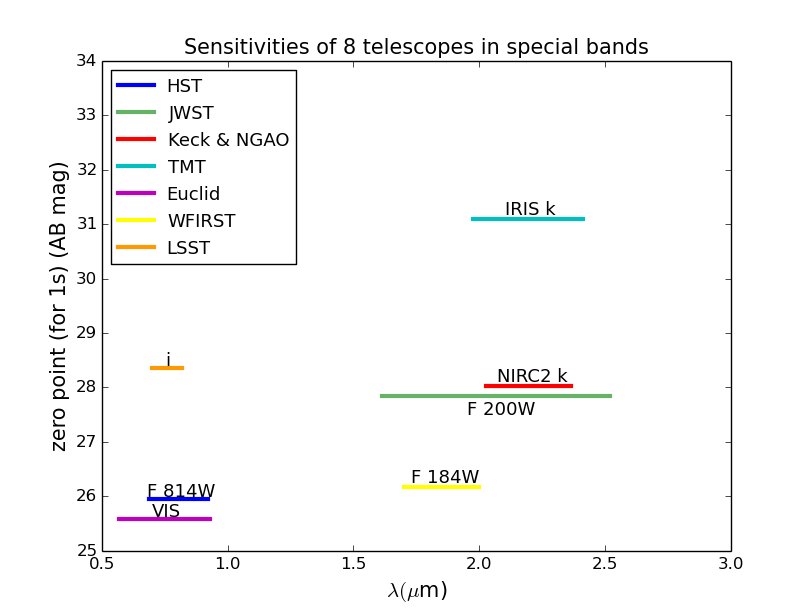
\includegraphics[width=0.9\textwidth]{figures/wavelength_zp.png}
\end{center}
\caption{Zero Points in AB magnitudes of HST (blue), JWST (green), Keck $\&$ NGAO (red), TMT (cyan), Euclid (magenta), WFIRST (yellow) and LSST (orange) in units of per second. Different color bars indicate the wavelength range of each telescope used in this work.}
\label{fig:zp_wavelength}
\end{figure}
% ================================================


% ================================================
\begin{figure}
\begin{center}
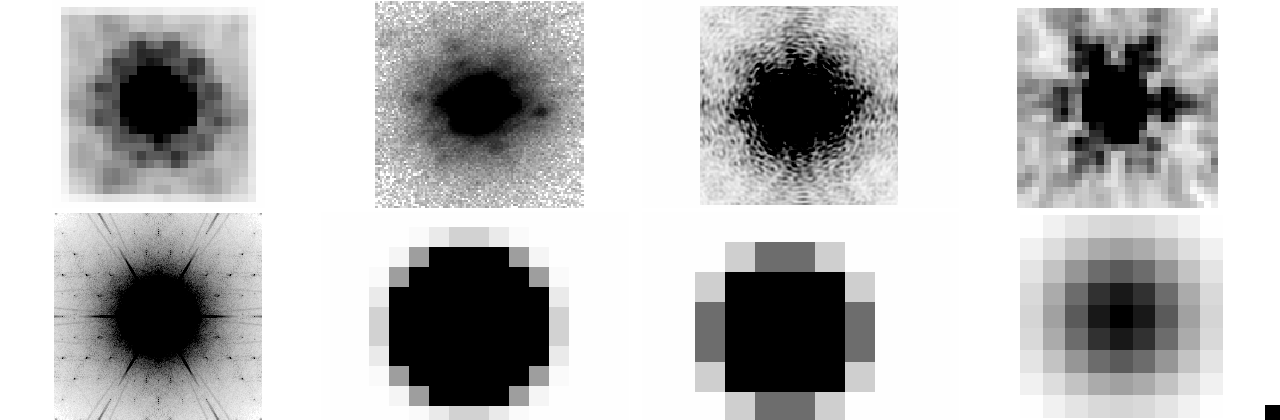
\includegraphics[width=1.0\textwidth]{figures/PSF_montage.png}
\end{center}
\caption{Gaussian PSF are used for Euclid, WFIRST, and LSST.}
\label{fig:PSF_montage}
\end{figure}
% =================================================



% ================================================
\begin{figure}
\begin{center}
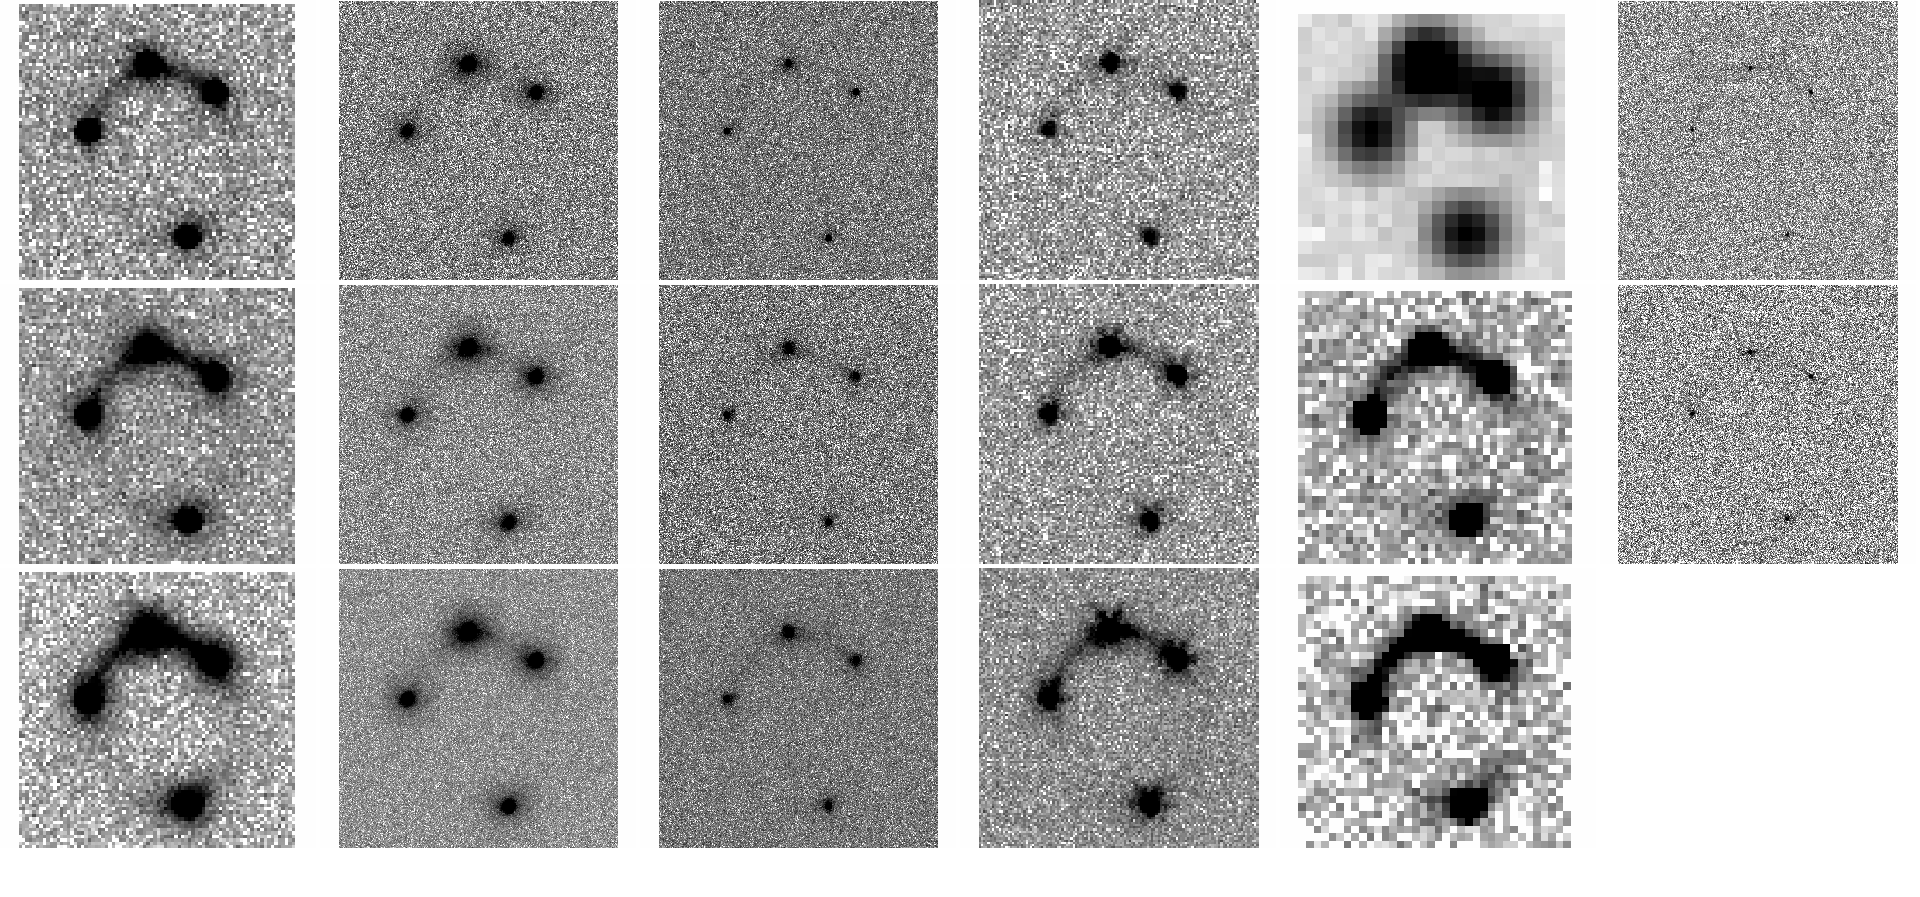
\includegraphics[width=1.0\textwidth]{figures/fainter_system_4QSOimages_all.png}
\end{center}
\caption{Simulated lens system results showing the fainter lens system (4 QSO images in the lens plane). The simulated image pixel scales are all 4$''$ $\times$ 4$''$. The first 4 columns, from left to right, represent HST, Keck, NGAO, and JWST; from top to bottom, correspond to 1/3 $\times$ good exposure time, good exposure time, and 3 $\times$ good exposure time ( See the definition of \textquotedblleft good exposure tine\textquotedblright\ in Section *.*). The fifth column include 3 survey detections by 3 different telescopes, from top to bottom, for LSST, Euclid, and WFIRST respectively. The last column is for TMT with 2 fixed exposure time: 360 seconds and 1080 seconds.}
\label{fig:fainter_4QSOimages_montage}
\end{figure}
% =================================================


% ================================================
\begin{figure}
\begin{center}
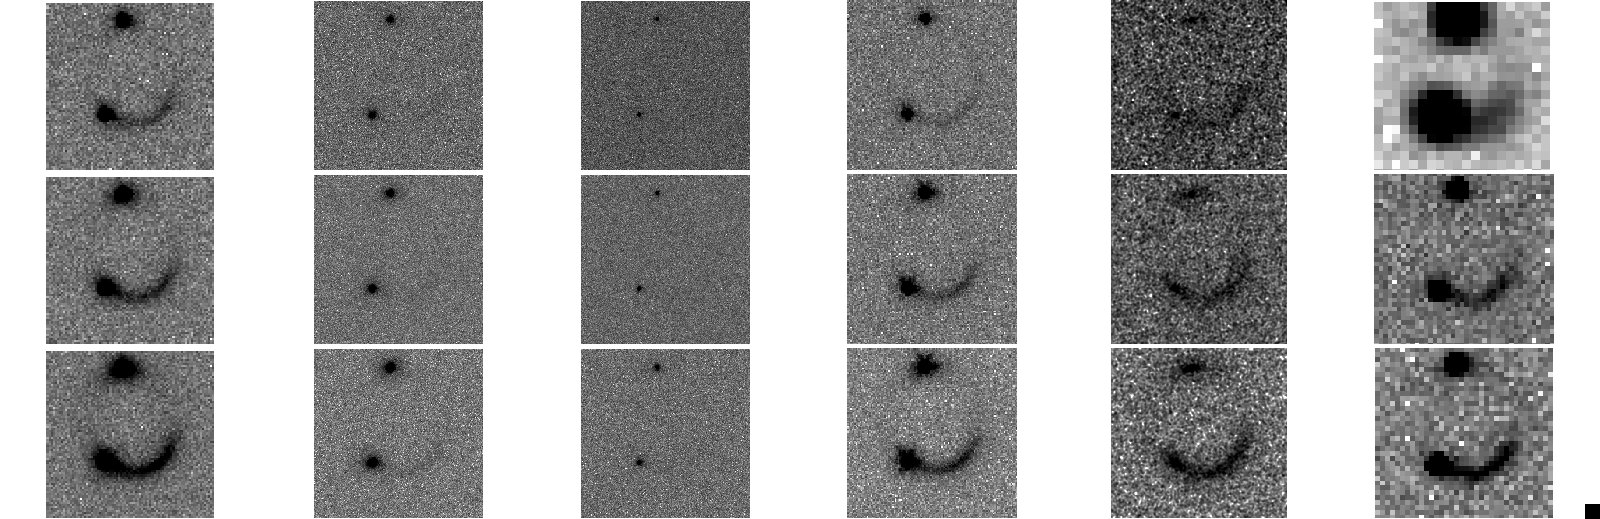
\includegraphics[width=1.0\textwidth]{figures/fainter_system_2QSOimages_all.png}
\end{center}
\caption{Same as Fig. 2, except that the simulated lens system results showing the fainter lens system (2 QSO images in the lens plane).}
\label{fig:fainter_2QSOimages_montage}
\end{figure}
% =================================================


% ================================================
\begin{figure}
\begin{center}
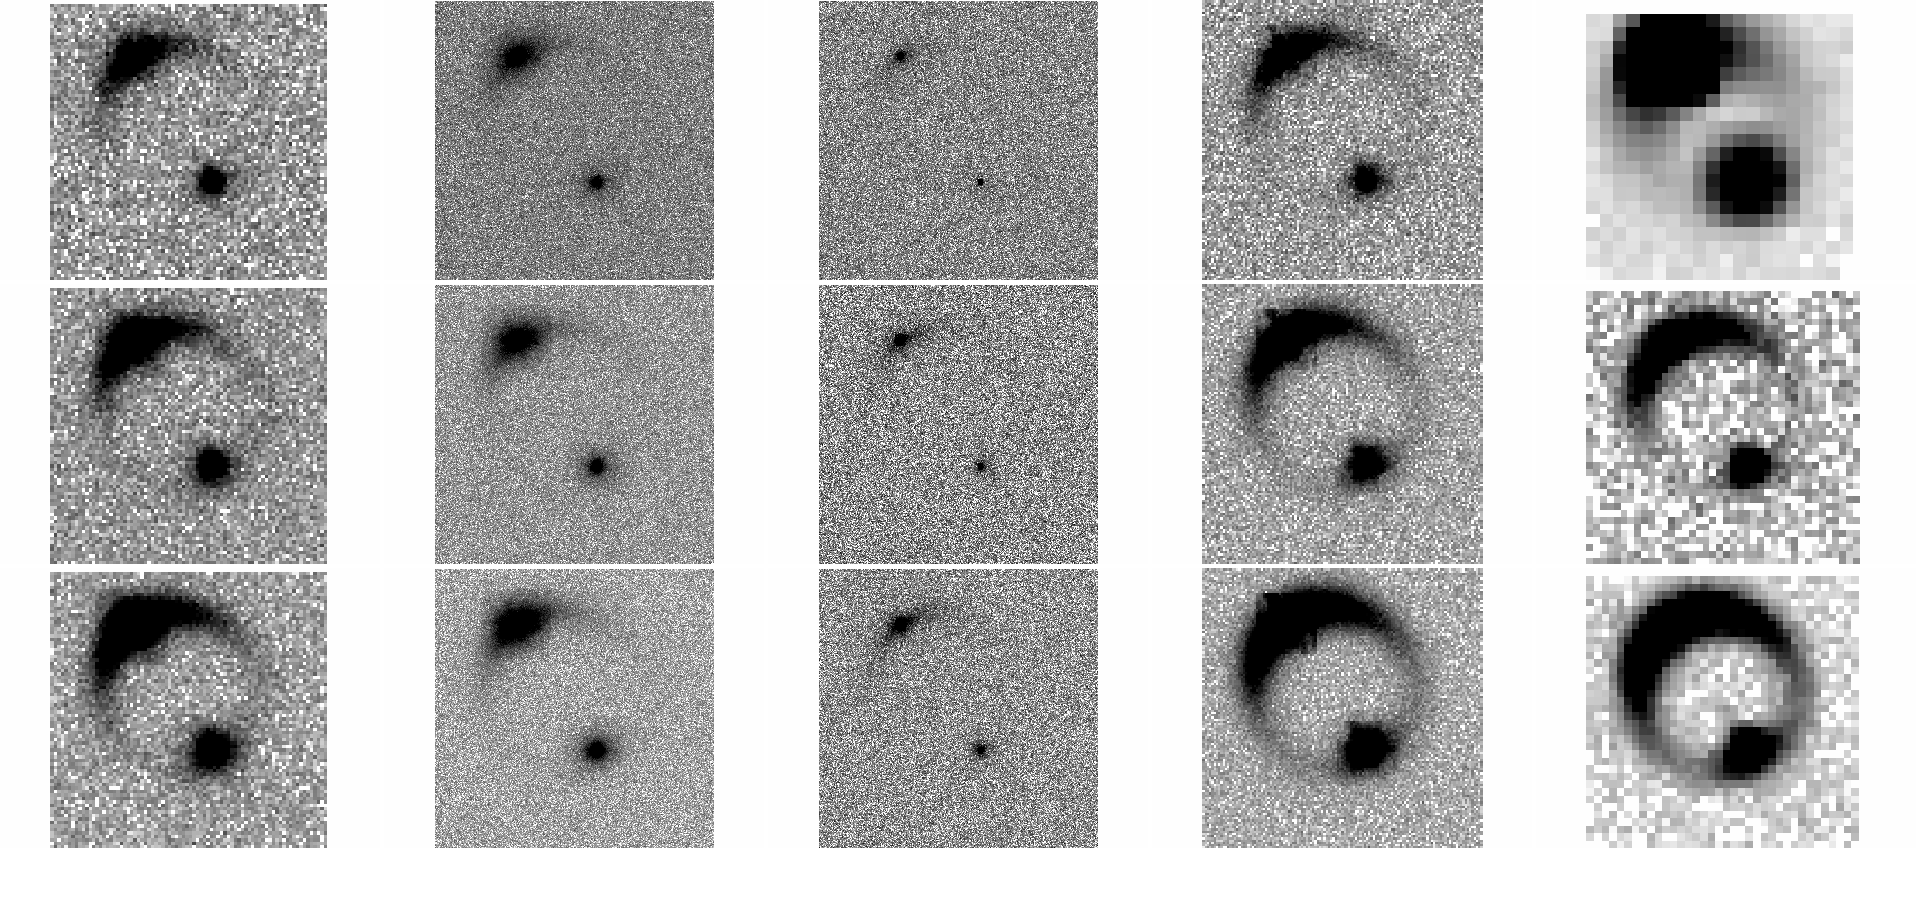
\includegraphics[width=1.0\textwidth]{figures/brighter_system_2QSOimages_all.png}
\end{center}
\caption{Simulated lens system results showing the brighter lens system (2 QSO images in the lens plane). The simulated image pixel scales are all 4$''$ $\times$ 4$''$. The first 3 columns, from left to right, present HST, Keck, and NGAO; from top to bottom, correspond to 1/3 $\times$ good exposure time, good exposure time, and 3 $\times$ good exposure time. The fourth column shows JWST with 3 fixed exposure time: 60 seconds, 180 seconds, and 540 seconds.The last column include 3 survey detections by 3 different telescopes, from top to bottom, for LSST, Euclid, and WFIRST respectively.}
\label{fig:brighter_2QSOimages_montage}
\end{figure}
% =================================================


% ================================================
\begin{figure}
\begin{center}
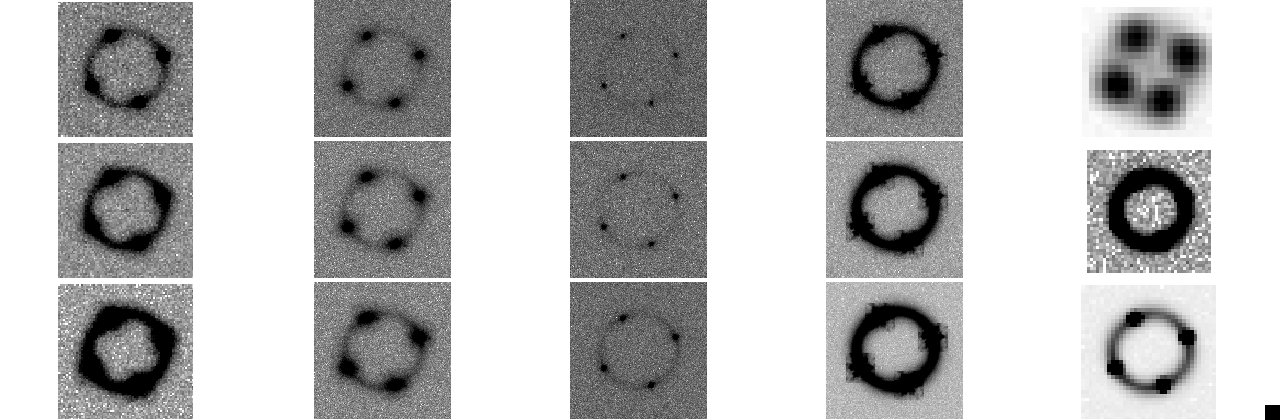
\includegraphics[width=1.0\textwidth]{figures/brighter_system_4QSOimages_all.png}
\end{center}
\caption{Same as Fig. 4, except that the simulated lens system results showing the brighter lens system (4 QSO images in the lens plane). The black spots in the center of the simulated images using HST, Euclid and WFIRST are from the efforts of strong signal pixels, so it's a \textquotedblleft ghost\textquotedblright\ image which can be ignored.}
\label{fig:brighter_4QSOimages_montage}
\end{figure}
% =================================================


% ==================================================
\begin{figure}
\begin{center}
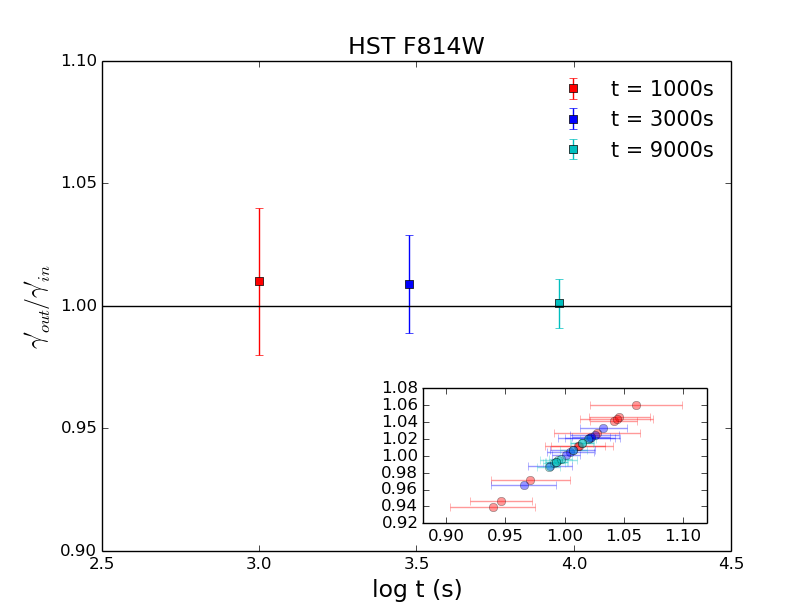
\includegraphics[width=0.48\textwidth]{figures/gamma_135949_4QSOimages_HST.png}
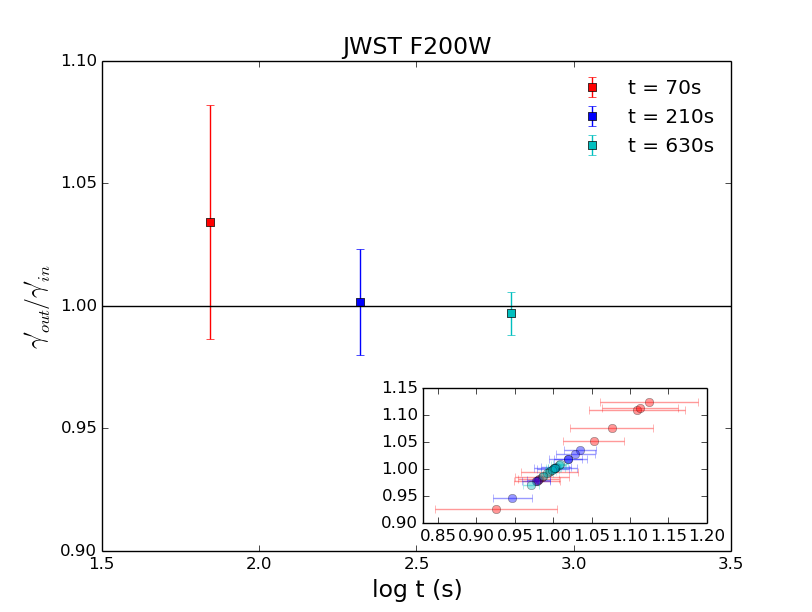
\includegraphics[width=0.48\textwidth]{figures/gamma_135949_4QSOimages_JWST.png} \\
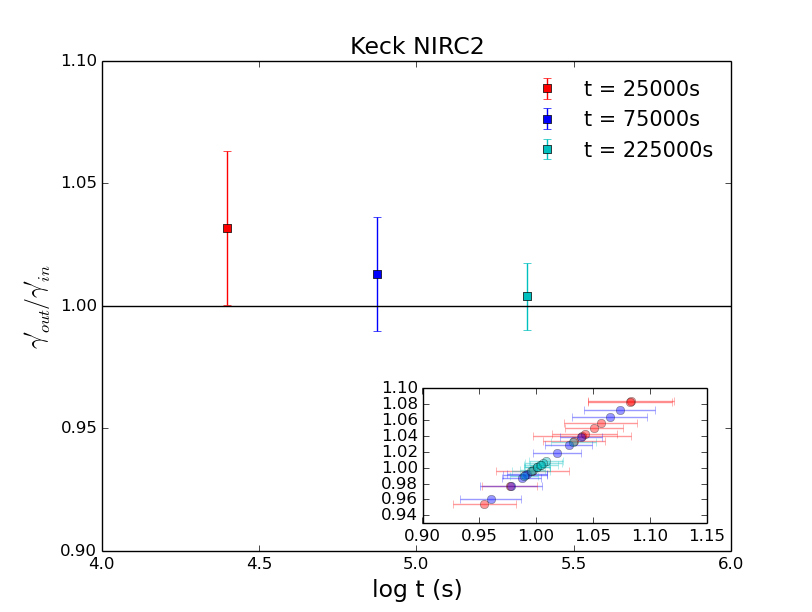
\includegraphics[width=0.48\textwidth]{figures/gamma_135949_4QSOimages_Keck.png}
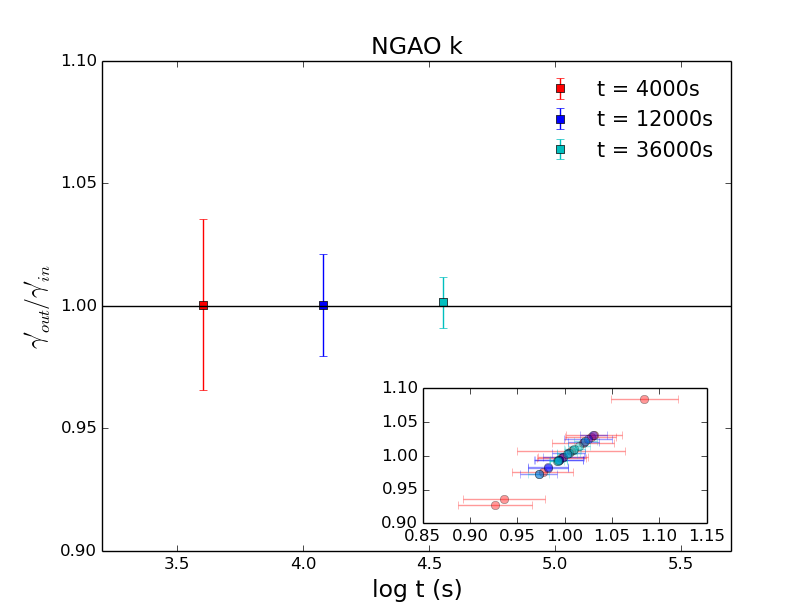
\includegraphics[width=0.48\textwidth]{figures/gamma_135949_4QSOimages_NGAO.png} \\
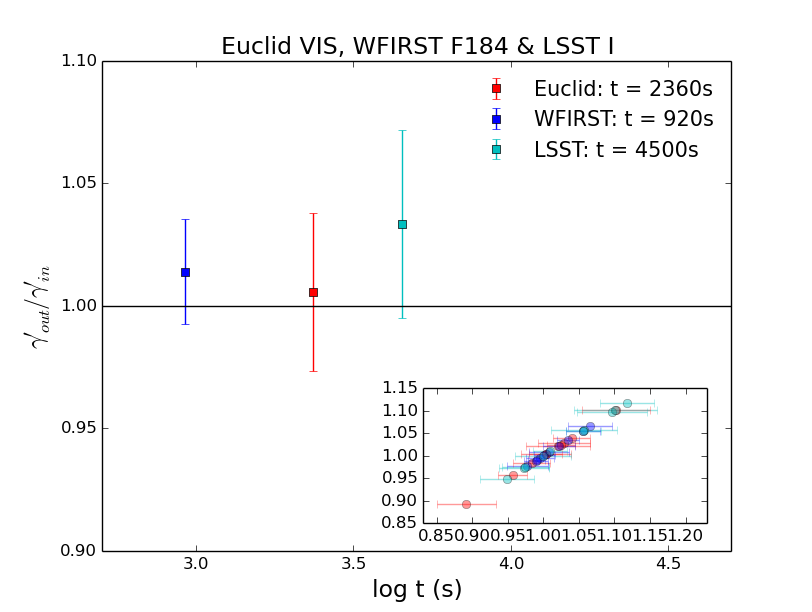
\includegraphics[width=0.48\textwidth]{figures/gamma_135949_4QSOimages_E_W_L.png}
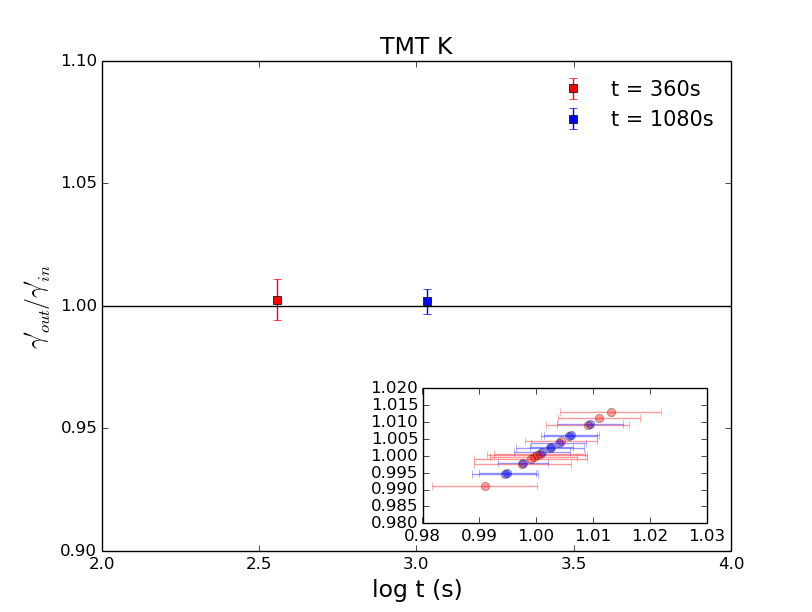
\includegraphics[width=0.48\textwidth]{figures/gamma_135949_4QSOimages_TMT.png}
\end{center}
\caption{The ability of recovering mass slope with respect to different exposure time for a variety of telescopes. This figure shows the fainter lens system with 4 QSO images in the lens plane. $\gamma'_{in}$ is the input SIE mass slope. $\gamma'_{out}$ is drawn from MCMC sampling based on the simulated images given $\gamma'_{in}$. The error bar represents 1$\sigma$ confidence range. The insert in each panel shows all 10 simulation results for each exposure time with the same color coding. Note that both axes represent $\gamma'_{out}/\gamma'_{in}$ whereas error bars are only shown on the x-axis for clarity.}
\label{fig:gamma_fainter_4QSOimages}
\end{figure}
% ======================================================


% ==================================================
\begin{figure}
\begin{center}
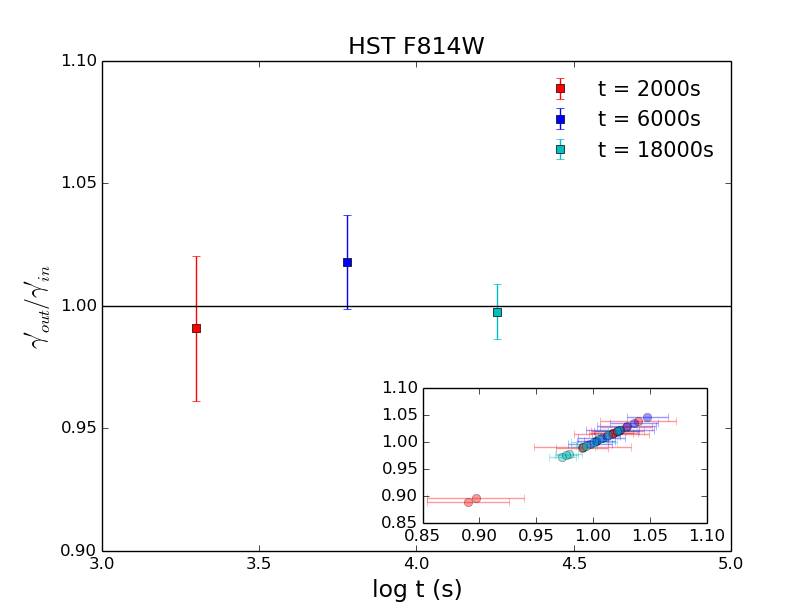
\includegraphics[width=0.48\textwidth]{figures/gamma_135949_anti_2QSOimages_HST.png}
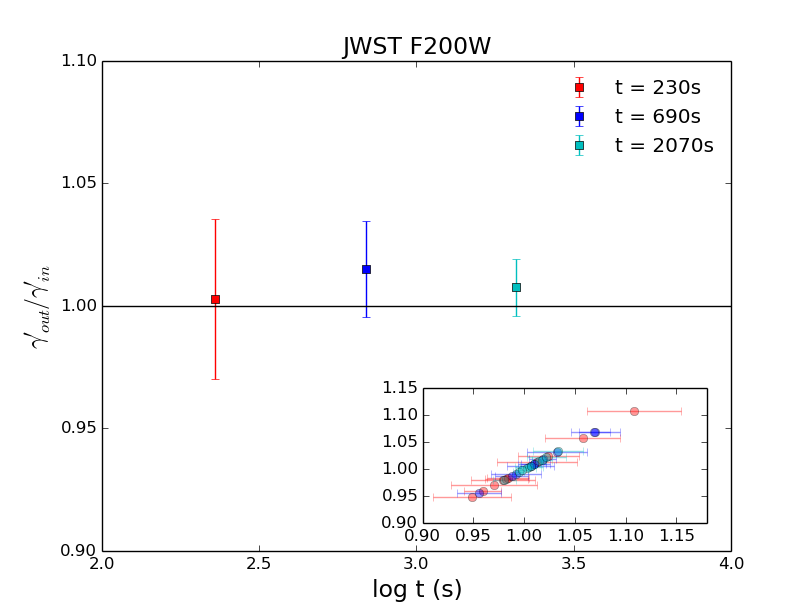
\includegraphics[width=0.48\textwidth]{figures/gamma_135949_anti_2QSOimages_JWST.png} \\
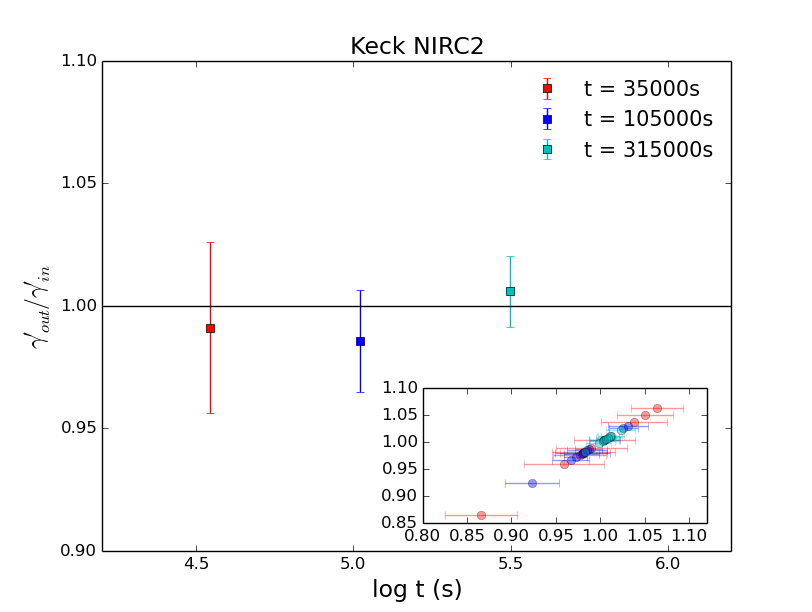
\includegraphics[width=0.48\textwidth]{figures/gamma_135949_anti_2QSOimages_Keck.png}
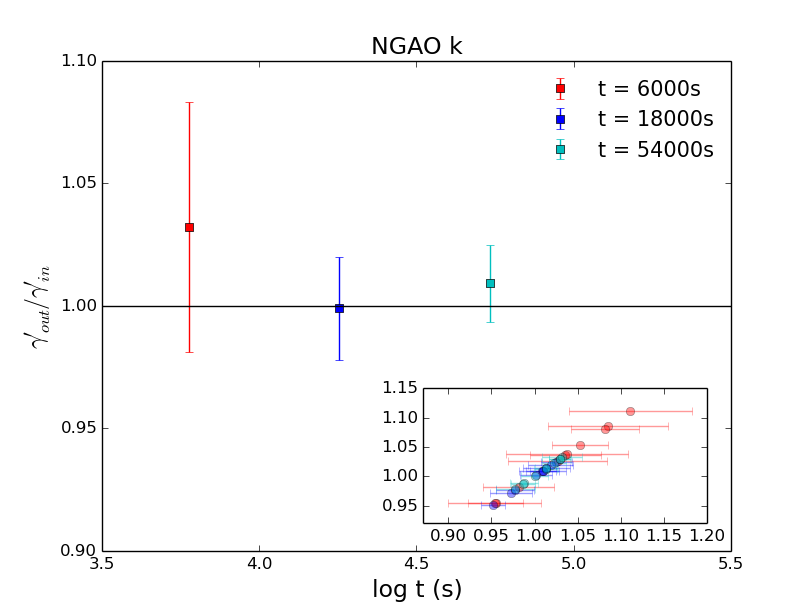
\includegraphics[width=0.48\textwidth]{figures/gamma_135949_anti_2QSOimages_NGAO.png} \\
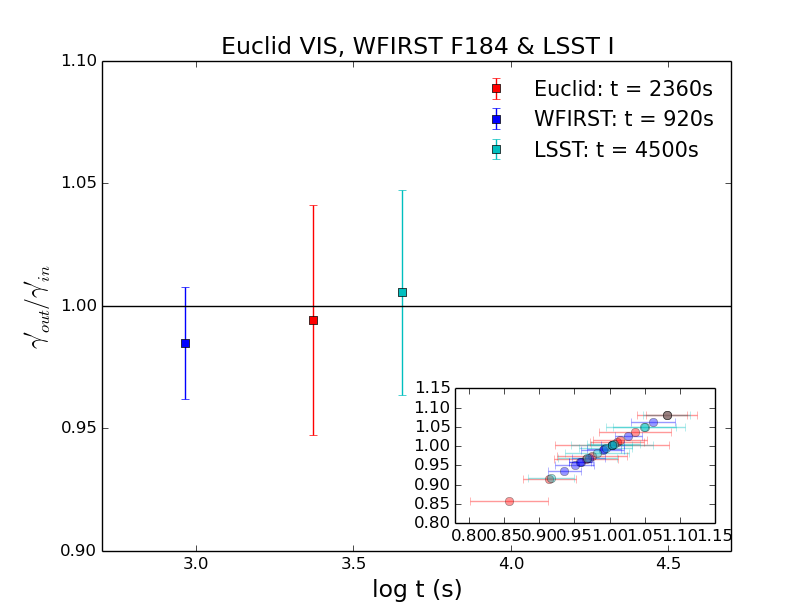
\includegraphics[width=0.48\textwidth]{figures/gamma_135949_anti_2QSOimages_EWL.png}
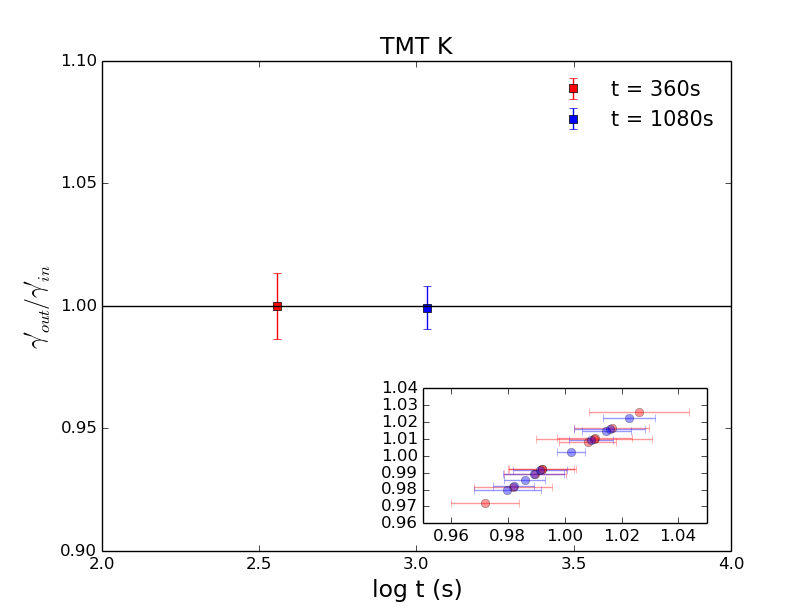
\includegraphics[width=0.48\textwidth]{figures/gamma_135949_anti_2QSOimages_TMT.png}
\end{center}
\caption{Same as Fig. 6, except that this figure is shown for the fainter lens system with 2 QSO images in the lens plane.}
\label{fig:gamma_fainter_2QSOimages}
\end{figure}
% ======================================================


% ==================================================
\begin{figure}
\begin{center}
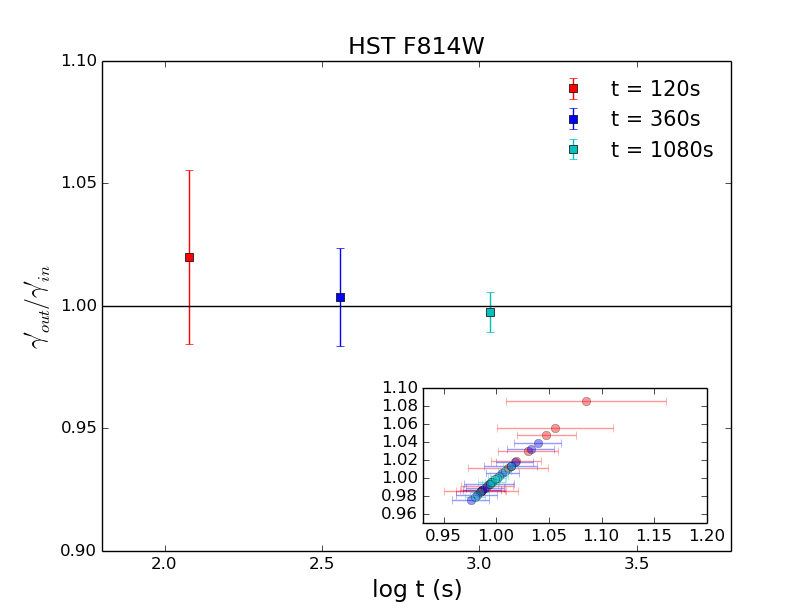
\includegraphics[width=0.48\textwidth]{figures/gamma_0330_2QSOimages_HST.png}
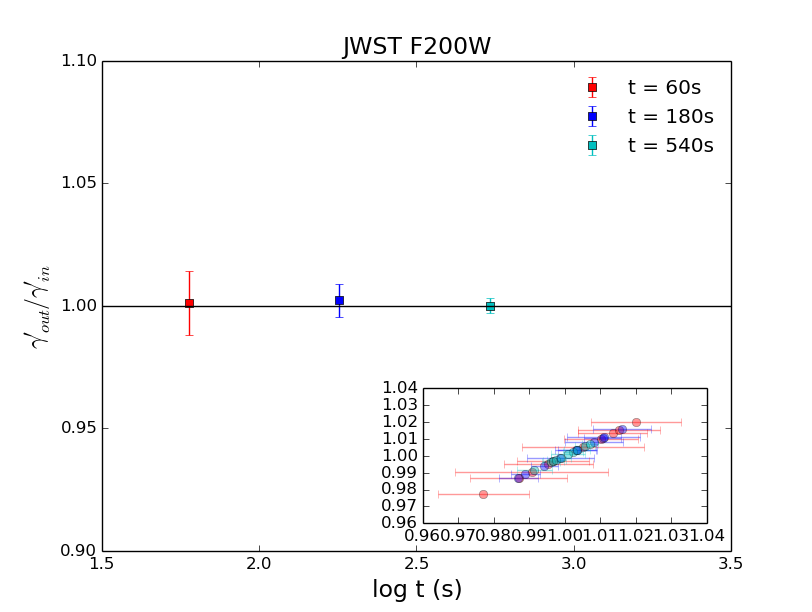
\includegraphics[width=0.48\textwidth]{figures/gamma_0330_2QSOimages_JWST.png} \\
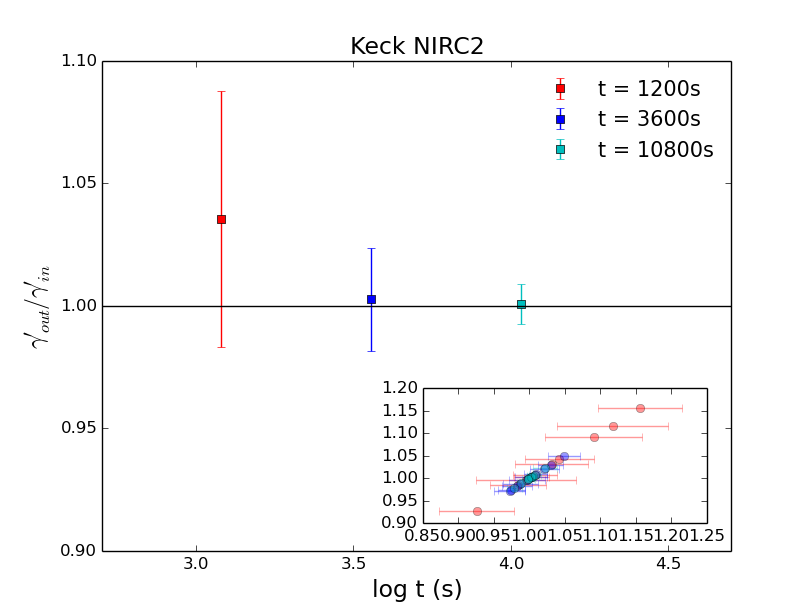
\includegraphics[width=0.48\textwidth]{figures/gamma_0330_2QSOimages_Keck.png}
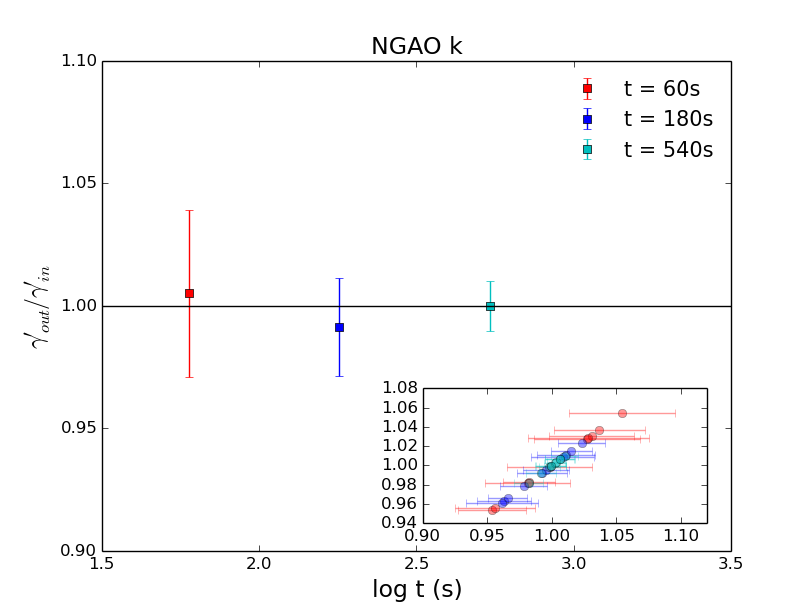
\includegraphics[width=0.48\textwidth]{figures/gamma_0330_2QSOimages_NGAO.png} \\
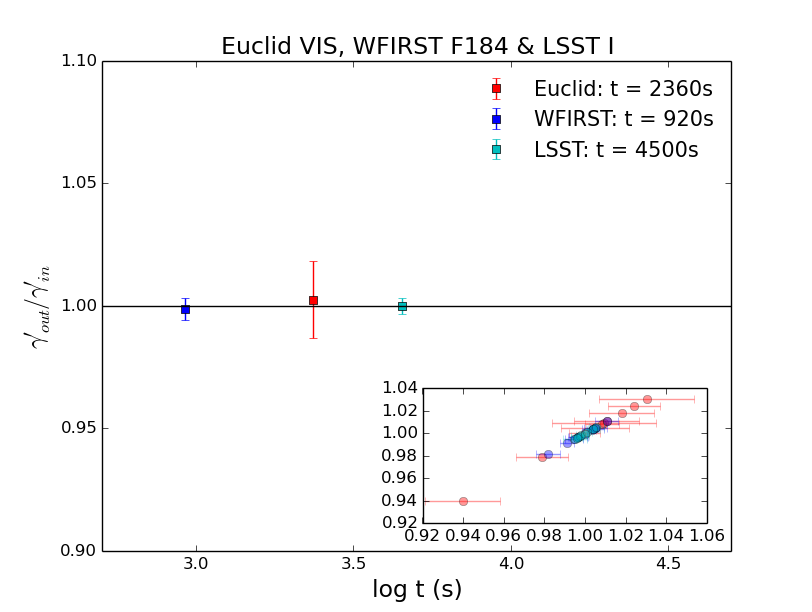
\includegraphics[width=0.48\textwidth]{figures/gamma_0330_2QSOimages_E_W_L.png}
\end{center}
\caption{Same as Fig. 6, except that this figure is shown for the brighter lens system with 2 QSO images in the lens plane.} 
\label{fig:gamma_brighter_2QSOimages}
\end{figure}
% ======================================================


% ==================================================
\begin{figure}
\begin{center}
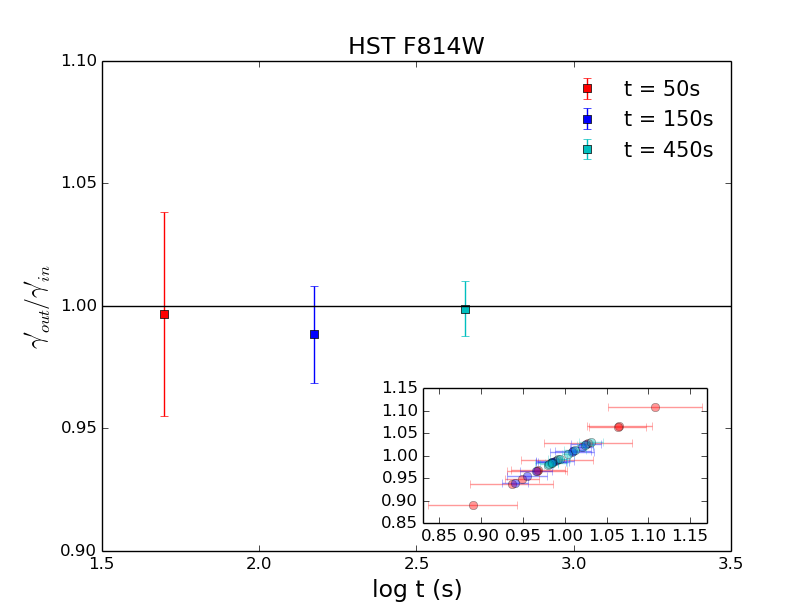
\includegraphics[width=0.48\textwidth]{figures/gamma_0330_anti_4QSOimages_HST.png}
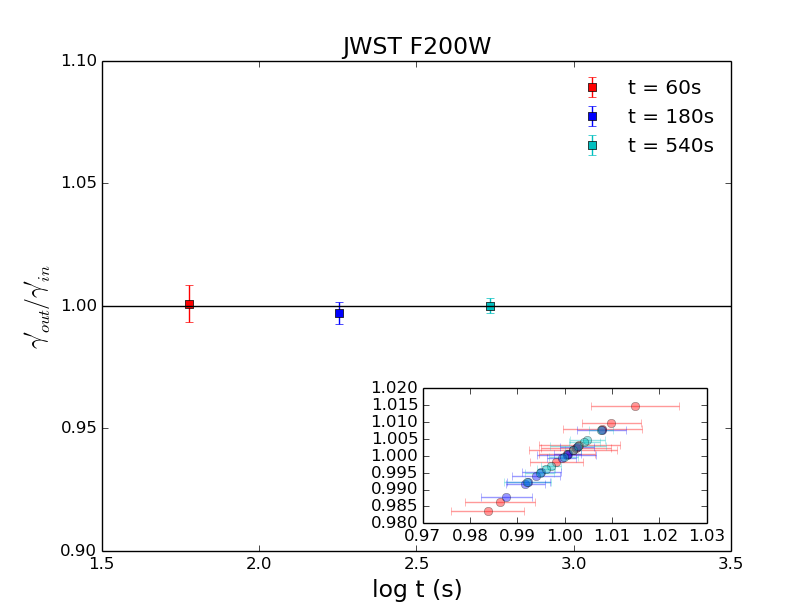
\includegraphics[width=0.48\textwidth]{figures/gamma_0330_anti_4QSOimages_JWST.png} \\
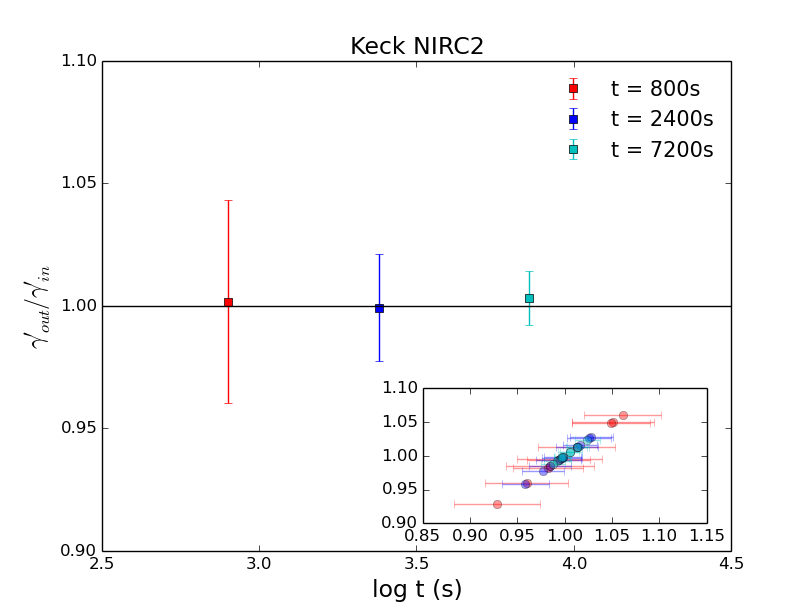
\includegraphics[width=0.48\textwidth]{figures/gamma_0330_anti_4QSOimages_Keck.png}
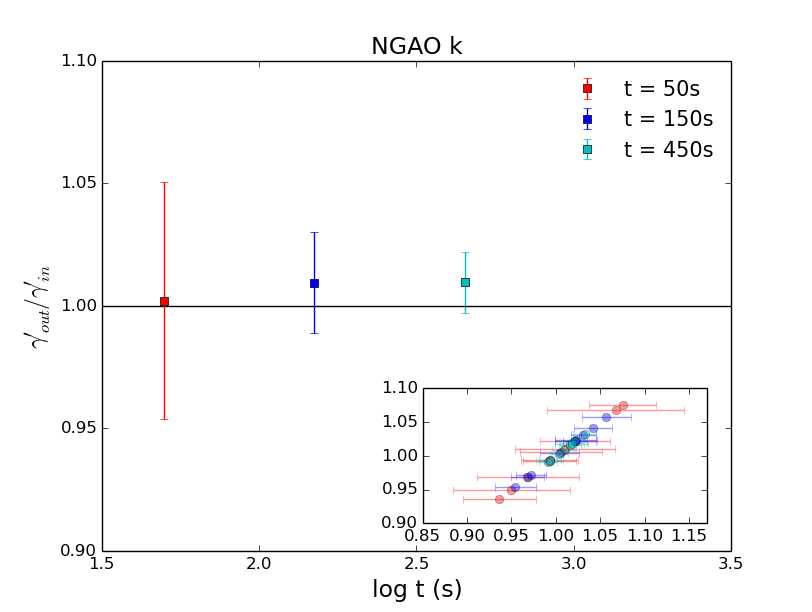
\includegraphics[width=0.48\textwidth]{figures/gamma_0330_anti_4QSOimages_NGAO.png} \\
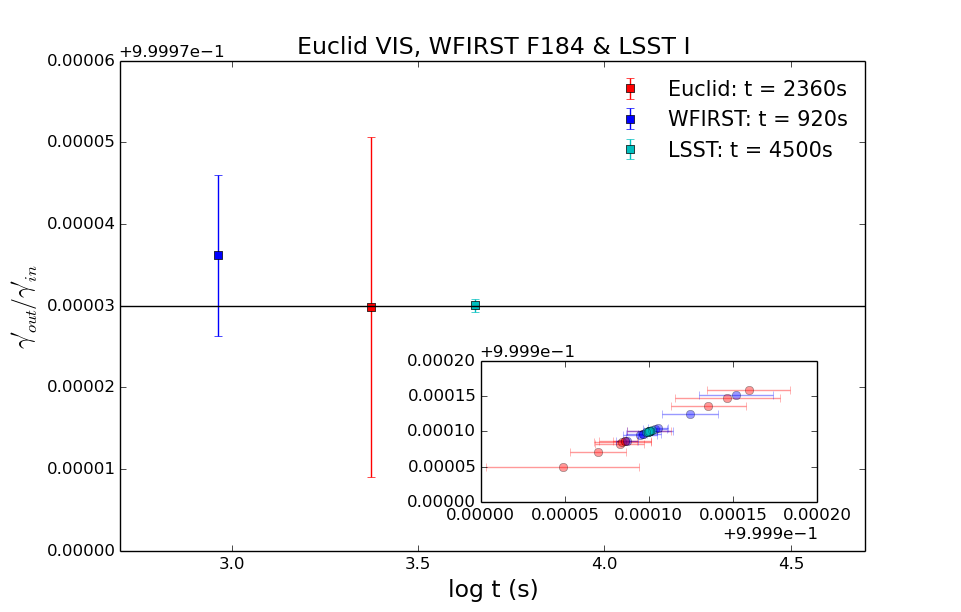
\includegraphics[width=0.48\textwidth]{figures/gamma_0330_anti_4QSOimages_EWL.png}
\end{center}
\caption{Same as Fig. 6, except that this figure is shown for the brighter lens system with 4 QSO images in the lens plane.}
\label{fig:gamma_brighter_4QSOimages}
\end{figure}
% ======================================================

\end{document}


\subsection{Selected Realistic Lens Systems}
For wider analysis we plan to We choose a lens from the Sloan Lens ACS Survey (SLACS; Bolton et al. 2008 \cite{2008ApJ...682..964B}; Auger et al. 2009 \cite{2009ApJ...705.1099A})